\usetikzlibrary{positioning}
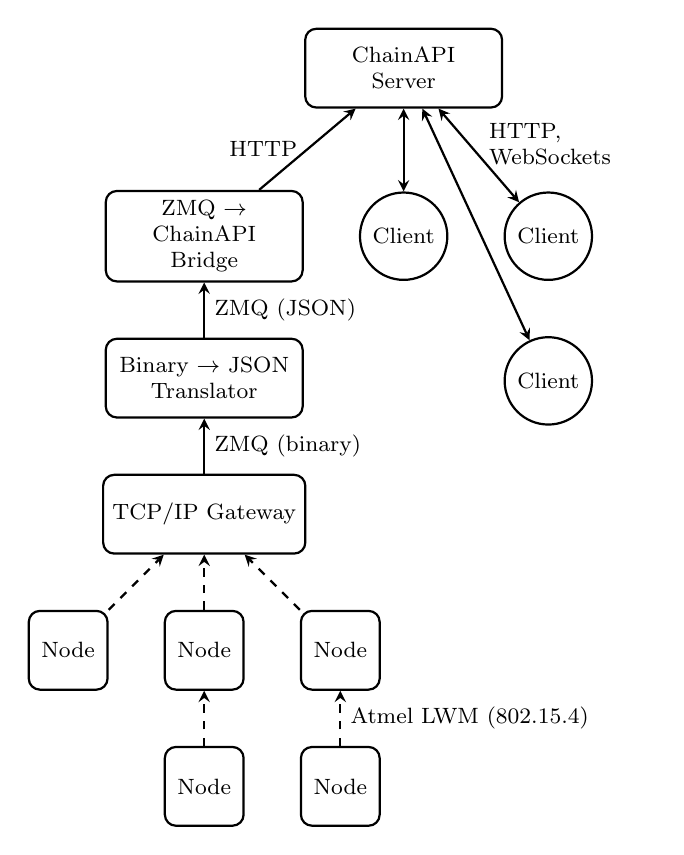
\begin{tikzpicture}[
	sensornode/.style={
		shape=rectangle,
		draw,
		minimum size=10mm,
		rounded corners,
	},
	gateway/.style={
		shape=rectangle,
		draw,
		rounded corners,
		minimum width=25mm,
		minimum height=10mm,
	},
	server/.style={
		shape=rectangle,
		draw,
		rounded corners,
		minimum width=25mm,
		minimum height=10mm,
		text width=22mm,
		align=center,
	},
	client/.style={
		shape=circle,
		draw
	},
	>=stealth,
	->,
	thick,
	font=\footnotesize,
	node distance=7mm,
]
% draw the bounding rectangle
%\draw (0,0) rectangle (8.45, 10);

\node (n4) [sensornode] at (2.5,1) {Node};
\node (n5) [sensornode, right=of n4] {Node};
\node (n7) [sensornode, above=of n4] {Node};
\node (n6) [sensornode, left=of n7] {Node};
\node (n8) [sensornode, right=of n7] {Node};
\node (gateway) [gateway, above=of n7] {TCP/IP Gateway};
\node (zmq server) [server, above=of gateway] {Binary $\to$ JSON Translator};
\node (zmq json server) [server, above=of zmq server] {ZMQ $\to$ ChainAPI\\Bridge};

\node (client1)[client, right=of zmq json server] {Client};
\node (client2)[client, right=of client1] {Client};
\node (client3)[client, below=of client2] {Client};
\node (chain server) [server, above =of client1, yshift=10] {ChainAPI Server};

\draw[dashed] (n4) -- (n7);
\draw[dashed] (n5) -- node[right] {Atmel LWM (802.15.4)}(n8);
\draw[dashed] (n6) -- (gateway);
\draw[dashed] (n7) -- (gateway);
\draw[dashed] (n8) -- (gateway);

\draw (gateway) -- node[right] {ZMQ (binary)} (zmq server);
\draw (zmq server) -- node[right] {ZMQ (JSON)} (zmq json server);
\draw (zmq json server) -- node[left] {HTTP} (chain server);
\draw[<->] (client1) -- (chain server);
\draw[<->] (client2) -- node[right, text width=2cm, yshift=1.5mm] {HTTP, \\WebSockets} (chain server);
\draw[<->] (client3) -- (chain server);
\end{tikzpicture}
